\documentclass[12pt]{article}
\usepackage{graphicx}
\usepackage{xcolor}
\usepackage{geometry}
\geometry{margin=1in}

\begin{document}

\begin{center}
\includegraphics[width=0.3\textwidth]{iiitb_logo.png.jpg}
\end{center}

\vspace{0.5cm}

\begin{center}
{\Large \textbf{Harshita N Kumar}} \\
ID: COMETFWC052
\end{center}

\vspace{0.8cm}

\begin{center}
{\Large \textcolor{blue}{\textbf{GATE Question no. 41}}}
\end{center}

{\color{blue}\section*{Question}}

For any set of inputs A and B, the following circuits give the same output $Q$, except one. Which one is it?

\vspace{0.5cm}

\begin{center}
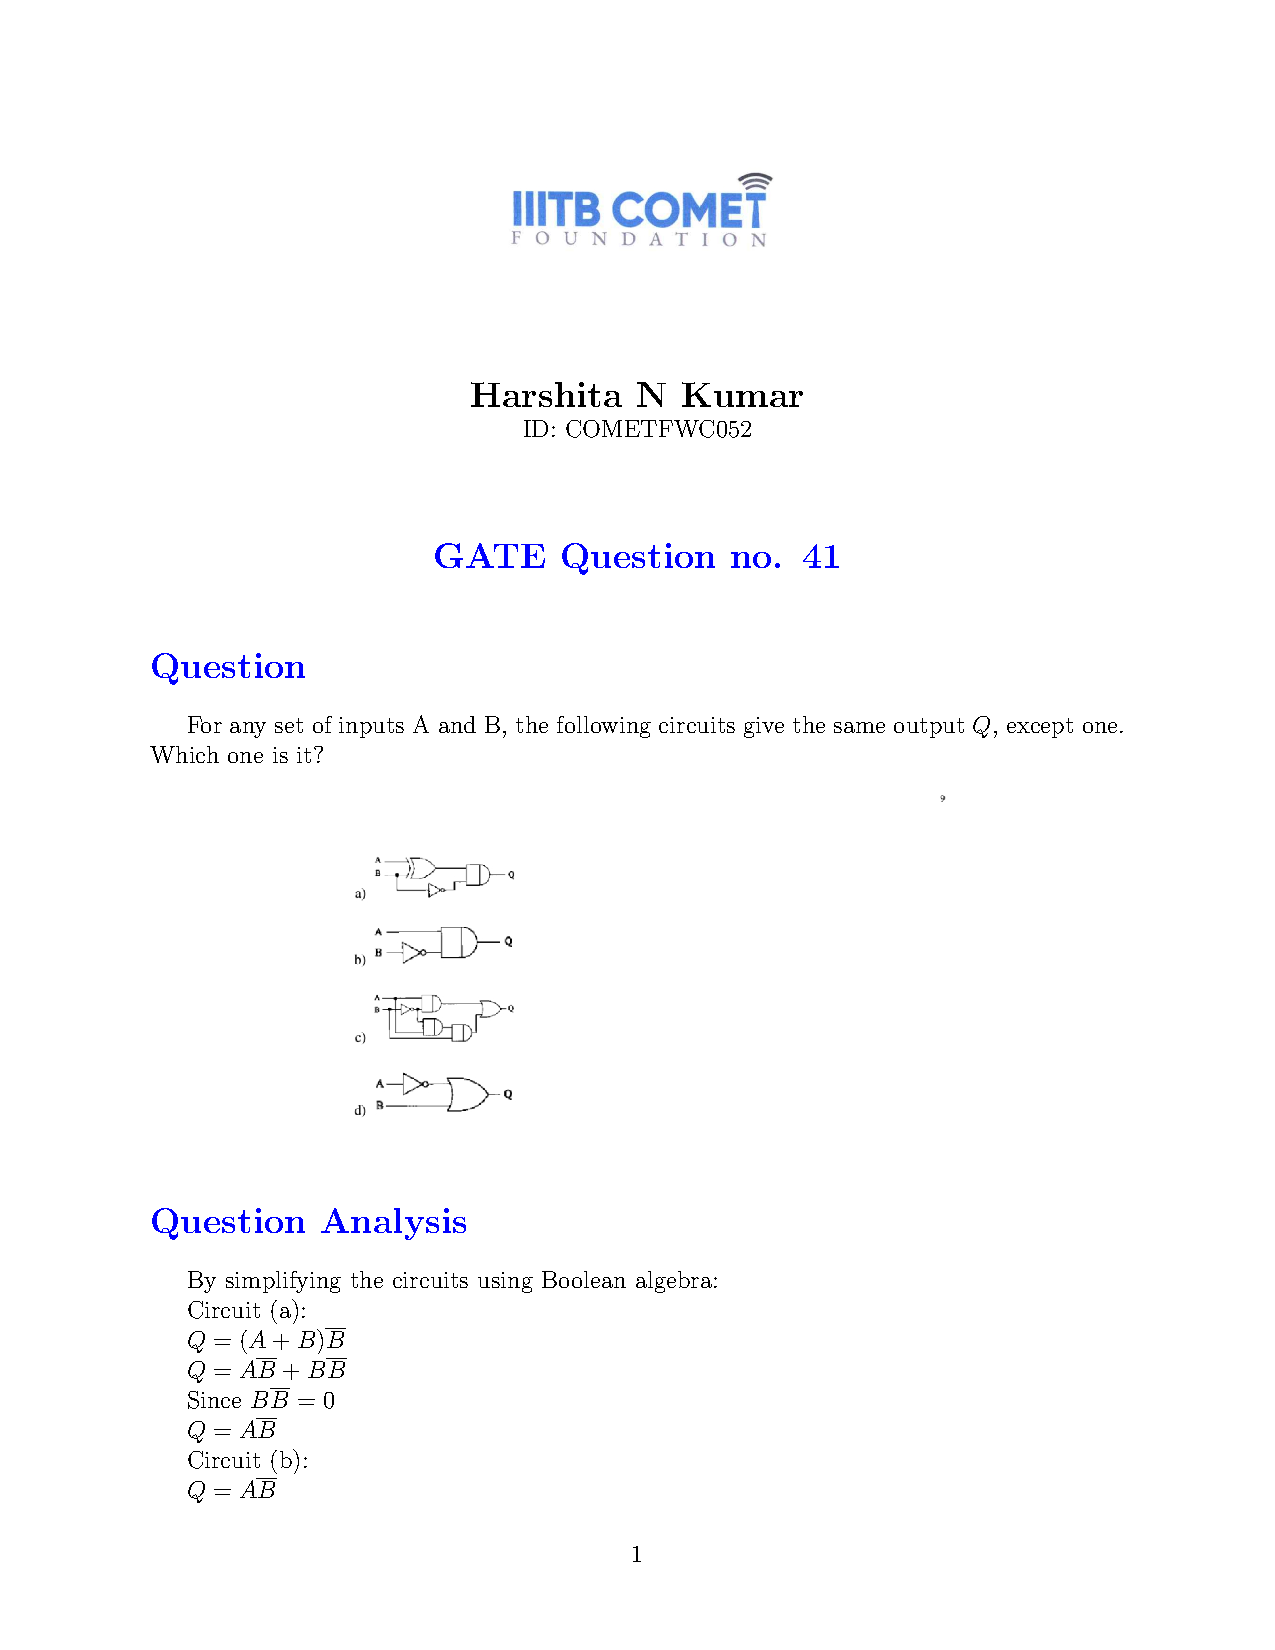
\includegraphics[width=0.75\textwidth]{gate_q41.jpg}
\end{center}

{\color{blue}\section*{Question Analysis}}

By simplifying the circuits using Boolean algebra:

Circuit (a):

$Q = (A + B)\overline{B}$

$Q = A\overline{B} + B\overline{B}$

Since $B\overline{B} = 0$

$Q = A\overline{B}$

Circuit (b):

$Q = A\overline{B}$

Circuit (c):

$Q = A\overline{B}$

Circuit (d):

$Q = \overline{A} + B$

Hence circuits (a), (b), and (c) produce identical outputs.

Circuit (d) produces a different output.

Correct Answer: (d)

{\color{blue}\section*{Theoretical Background}}

Boolean algebra is the mathematical foundation of digital electronics.

Important laws used:

Complement Law: $A\overline{A} = 0$

Identity Law: $A + 0 = A$

Distributive Law: $A(B + C) = AB + AC$

The simplified function is:

$Q = A\overline{B}$

This means output is HIGH only when:

$A = 1$ and $B = 0$

{\color{blue}\section*{Truth Table}}

\begin{center}
\begin{tabular}{|c|c|c|c|}
\hline
A & B & $A\overline{B}$ & $\overline{A}+B$ \\
\hline
0 & 0 & 0 & 1 \\
0 & 1 & 0 & 1 \\
1 & 0 & 1 & 0 \\
1 & 1 & 0 & 1 \\
\hline
\end{tabular}
\end{center}

The outputs clearly show that circuit (d) differs.


\begin{itemize}
\item Arduino UNO
\item IC 7447 (BCD to 7-segment decoder)
\item Common Anode 7-segment display
\item Breadboard
\item Jumper wires
\end{itemize}

{\color{blue}\section*{Pin Connections}}

\textbf{IC 7447 Connections}

Pin 16 $\rightarrow$ 5V \\
Pin 8 $\rightarrow$ GND

Control pins 3, 4, 5 $\rightarrow$ 5V

Pins 1 and 2 $\rightarrow$ GND

Pin 7 $\rightarrow$ Arduino Pin 9

\vspace{0.3cm}

\textbf{Arduino Inputs}

Pin 10 $\rightarrow$ A \\
Pin 11 $\rightarrow$ B

\vspace{0.3cm}

\textbf{7-Segment}

Common Anode $\rightarrow$ 5V

Segment pins connected from 7447 outputs through resistors.

{\color{blue}\section*{Logic Description}}

The Arduino provides inputs A and B.

The logical expression verified is:

$Q = A\overline{B}$

The output is displayed on a 7-segment display using IC 7447.

If $Q = 1$, display shows HIGH condition.  
If $Q = 0$, display shows LOW condition.

{\color{blue}\section*{Code Uploading Steps}}

1. Create a Platform IO project.

2. Write the code in main.cpp inside src folder.

3. Run:

\texttt{pio run}

4. Copy the generated .hex file to Arduino Droid folder.

5. Connect Arduino UNO using OTG cable.

6. Upload using "Upload Precompiled" option.

7. Observe output and verify $Q = A\overline{B}$.

{\color{blue}\section*{Experimental Truth Table}}

\begin{center}
\begin{tabular}{|c|c|c|}
\hline
A & B & Observed Output \\
\hline
0 & 0 & 0 \\
0 & 1 & 0 \\
1 & 0 & 1 \\
1 & 1 & 0 \\
\hline
\end{tabular}
\end{center}

{\color{blue}\section*{Hardware Implementation}}

\begin{center}
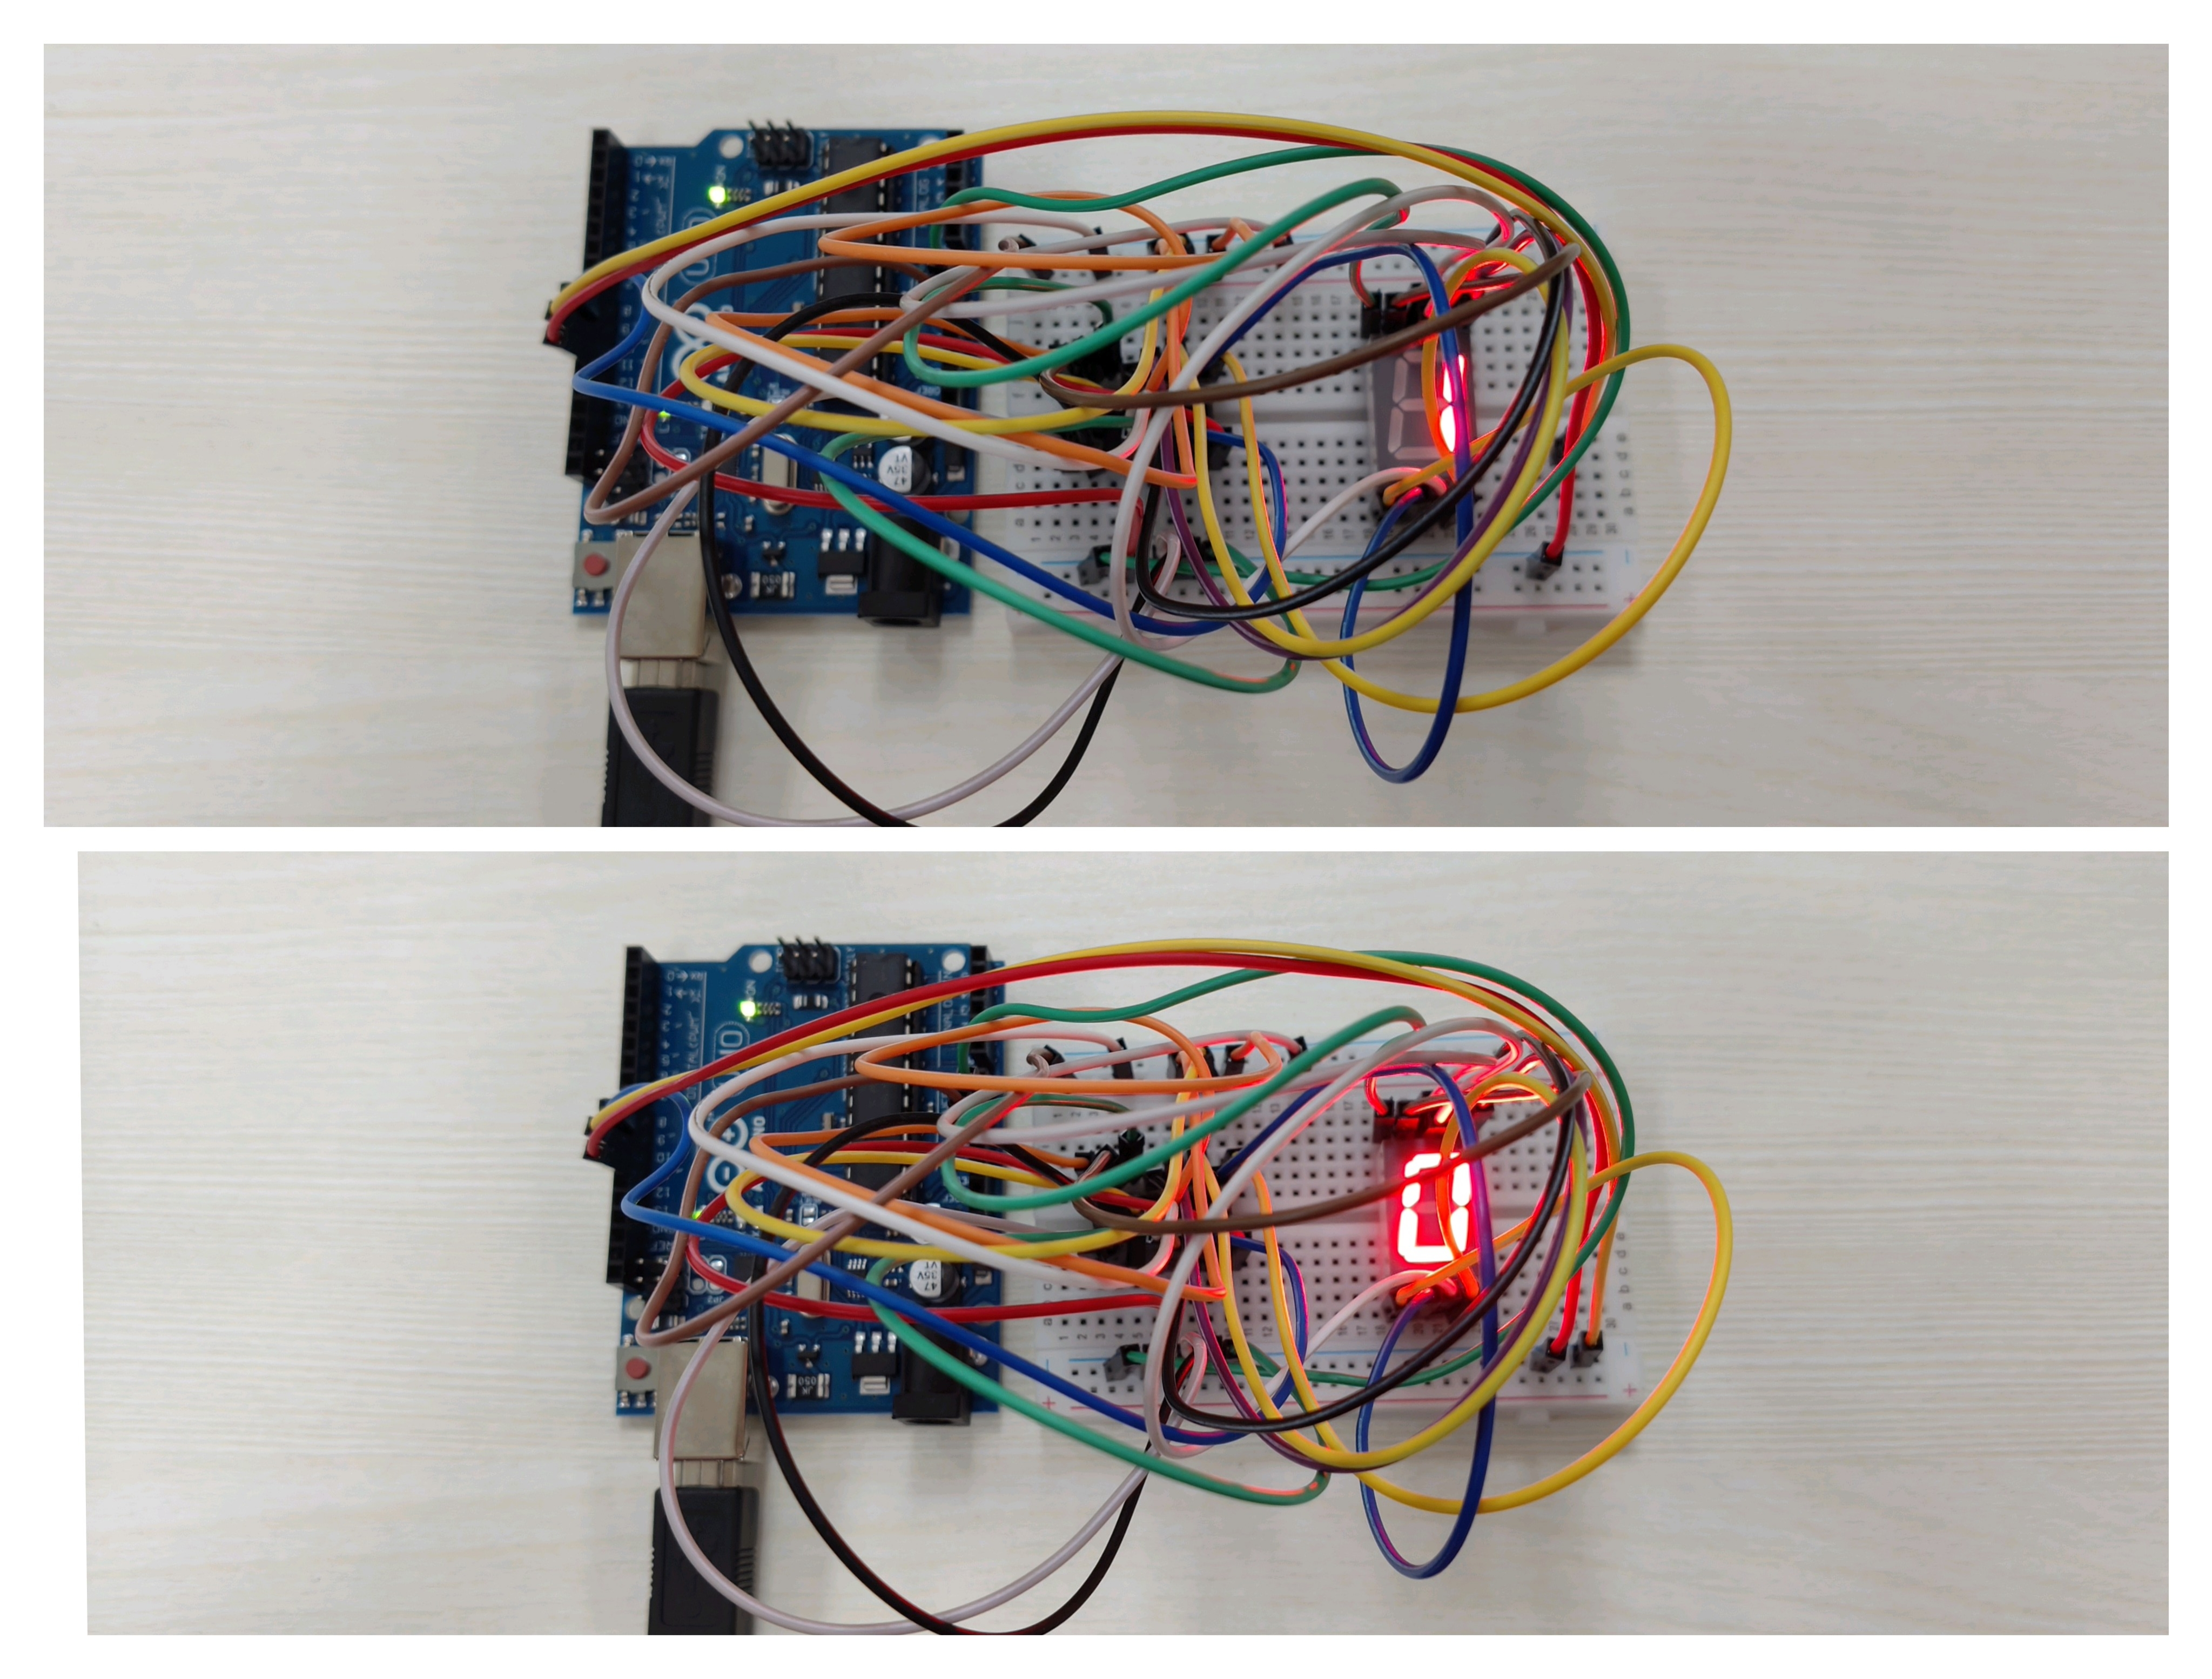
\includegraphics[width=0.8\textwidth]{hardware.jpg}
\end{center}

{\color{blue}\section*{Conclusion}}

From Boolean simplification, theoretical truth table, and hardware testing:

$Q = A\overline{B}$

Circuits (a), (b), and (c) produce same output.

Circuit (d) produces different output.

Hence the correct answer is:

\textbf{(d)}

\end{document}
